The tool I implemented, called \toolname, is a \textit{java-based} tool aimed at helping further developers during the testing process of their Android mobile applications. \\
For giving a cleaner and more understandable explanation of how \toolname\ works, I would like to split its key features into three main categories (which should also be executed in a sequential way, in order to exploit the whole \toolname's potentiality): 
\begin{enumerate}
\item the \textsc{testing} part is in charge of testing a given set of \textit{APKs}, reporting their testing results and extracting possible \textit{crashes} from the before generated testing logs; 

\item the \textsc{clustering} part investigates the similarity between the previous extracted crash logs, using different metrics and strategies, in order to collect they together and create a crash log \textit{bucket}; 

\item the \textsc{linking} part represents the core feature of \toolname. It pre-processes a set of given \textit{user reviews} as well as the set of the previously created crash logs, in order to prepare and "clean" them for the linking procedure.  Afterwards, it investigates whether it exists a correlation between the stack traces and the user feedbacks, with the aim to link, whether possible, the reviews with the crash logs. 
\end{enumerate}

\section{Testing}
%----------------- FDROID CRAWLER --------------
First of all, if there is no a set of \textit{APKs} yet, \toolname\ can be exploited for downloading the needed mobile applications from the \textit{F-Droid API\footnote{LINK API}}. In this direction, as shown in the picture \ref{testing}, the component \textsc{fdroid crawler}, is first in charge of  parsing a static structured file, which contains a set of android packages names. 
The path of this file is given in the \textsc{configuration manager}, which contains a set of static properties that get elaborated by \toolname. Second, \textsc{fdroid crawler} searches and then extracts a set of \textit{HTTP links} for those android packages that have been found on the API. Afterwards, it builds the correct \textit{HTTP requests} and finally starts the downloading process, saving the returned \textit{APKs} in a given directory.

%-------------- CONFIGURATION ENVIRONMENT--------------
The first step was to build a set of \textit{APKs}, with which to perform the testing process. As said, this can be achieved using either \textsc{fdroid crawler} or can also be manually set. Now, the second step is to prepare and configure the testing environment. 
All the parameters needed for starting a testing session have to be specified in the \textsc{configuration manager}. Figure \ref{config}, shows an example of a simplified set of parameters which must be given a priori in order to launch a testing session. \newpage
\label{config}
\begin{lstlisting}[caption=A set of needed properties which get elaborated during the testing session]
/**
 * Testing session specifications
 */
MINUTES_PER_APP = 30
NR_OF_ITERATIONS
 
/**
* Testing logs directories
*/
MONKEY_DIR = Reports/MonkeyReports
SAPIENZ_DIR = Reports/SapienzReports

/**
 * Monkey parameters
 */
LOG_VERBOSITY = -v 
PACKAGE_ALLOWED = -p
NR_INJECTED_EVENTS = 5000
DELAY_BETWEEN_EVENTS = 10
PERCENTAGE_TOUCH_EVENTS = 15
PERCENTAGE_SYSTEM_EVENTS = 15
PERCENTAGE_MOTION_EVENTS = 15
IGNORE_CRASH = True

/**
* Sapienz parameters
*/
SEQUENCE_LENGTH_MIN = 20
SEQUENCE_LENGTH_MAX = 500
SUITE_SIZE = 5
POPULATION_SIZE = 50
OFFSPRING_SIZE = 50
GENERATION = 100
CXPB = 0.7
MUTPB = 0.3
\end{lstlisting}
The figure above represents a part of the \textsc{configuration manager}, where all the testing parameters for \monkey and \sapienz are specified. An in-depth explanation about these parameters concering \monkey and \sapienz can be found on \cite{monkey}, respectively on \cite{sapienz}.\\
In addition to them, the directories on which the generated testing logs are going to be stored must be given and


% TOODOOO
the automated tool with whom the testing is going to be performed must be made explicit. Indeed, it has to be specified as parameter in \textsc{main} \textit{args} (as mentioned before in the section \ref{sec:choicetool}, the tools which can be selected are either \monkey or \sapienz). \\
The last configuration step is to define on which kind of device (\textit{i.e}, a real device, such as a \textit{tablet} or a virtual device, such as an \textit{emulator}) the testing is going to be performed. \toolname\ supports different types of emulators or real devices running on different android API levels. However, in order to correctly execute \sapienz, the API level shall be the \textit{Android 4.4, KitKat}. 


%-----------LAUNCH A TESTING SESSION -----------




Once the configuration phase is terminated, \toolname\ is able to start the testing process. 
As shown in the picture \ref{testing},  

 %and installs them one by one during the testing phase. It installs them on one or more attached mobile devices and starts the automated testing phase. It stress the AUT using the automated testing tool specified as parameter in the \textit{Main} body  







Afterwards, \toolname\ stores the from these automated testing tools generated reports, it scans them and whether a bug occurred, it extracts the \textit{crash} from the documented \textit{stack trace} and accurately writes it on a new file, in order to differentiate stack traces without crashes

\section{Clustering}

\section{Linking}

\section{How to start \toolname}
First of all, a set of parameters and directories have to inserted in the static \textit{Configuration Manager} file.
% qui inserire la command-line

\begin{figure}[t]
\centering 
%	\vspace{-1.5mm} 
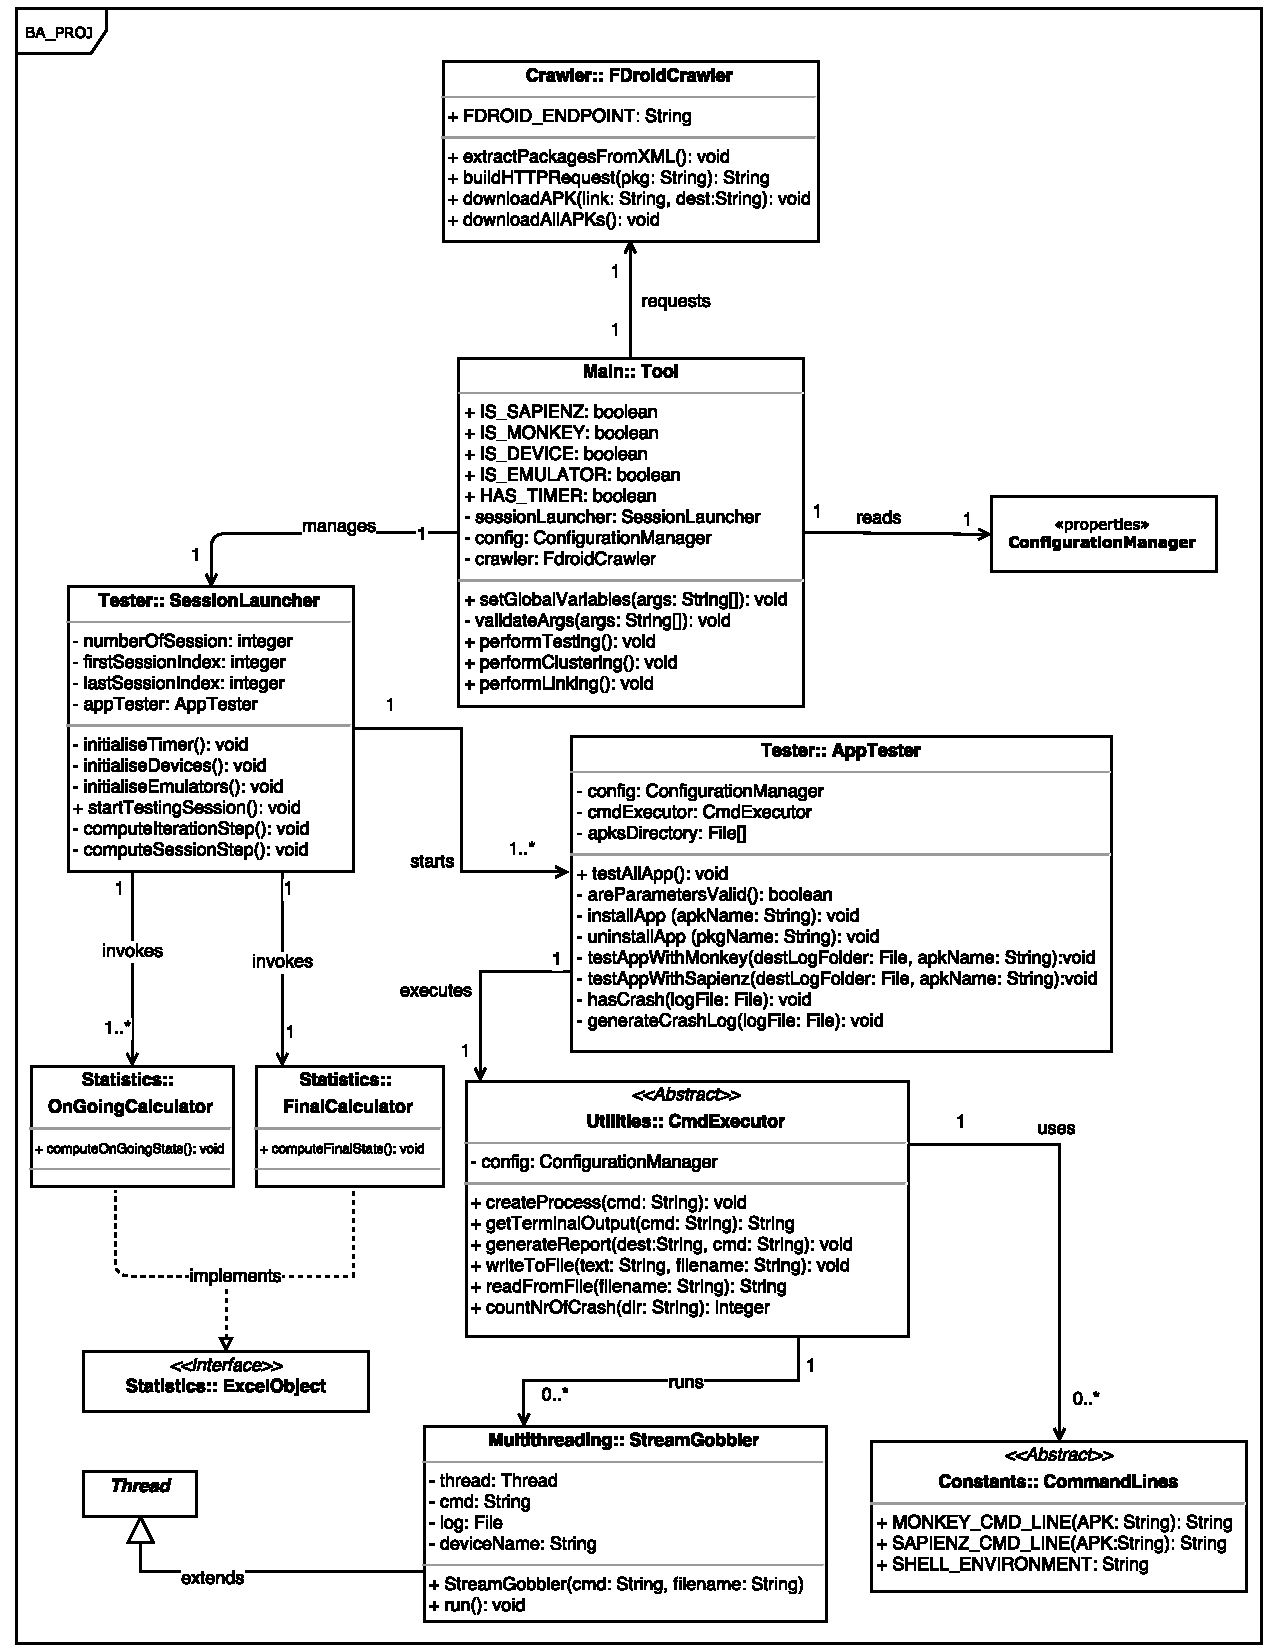
\includegraphics[width=\columnwidth]{diagrams/testing.pdf} 
\caption{Class Diagram of the testing part of the tool }
\label{testing}
\vspace{-3mm} 
\end{figure}



\begin{figure}[t]
\centering 
%	\vspace{-1.5mm} 
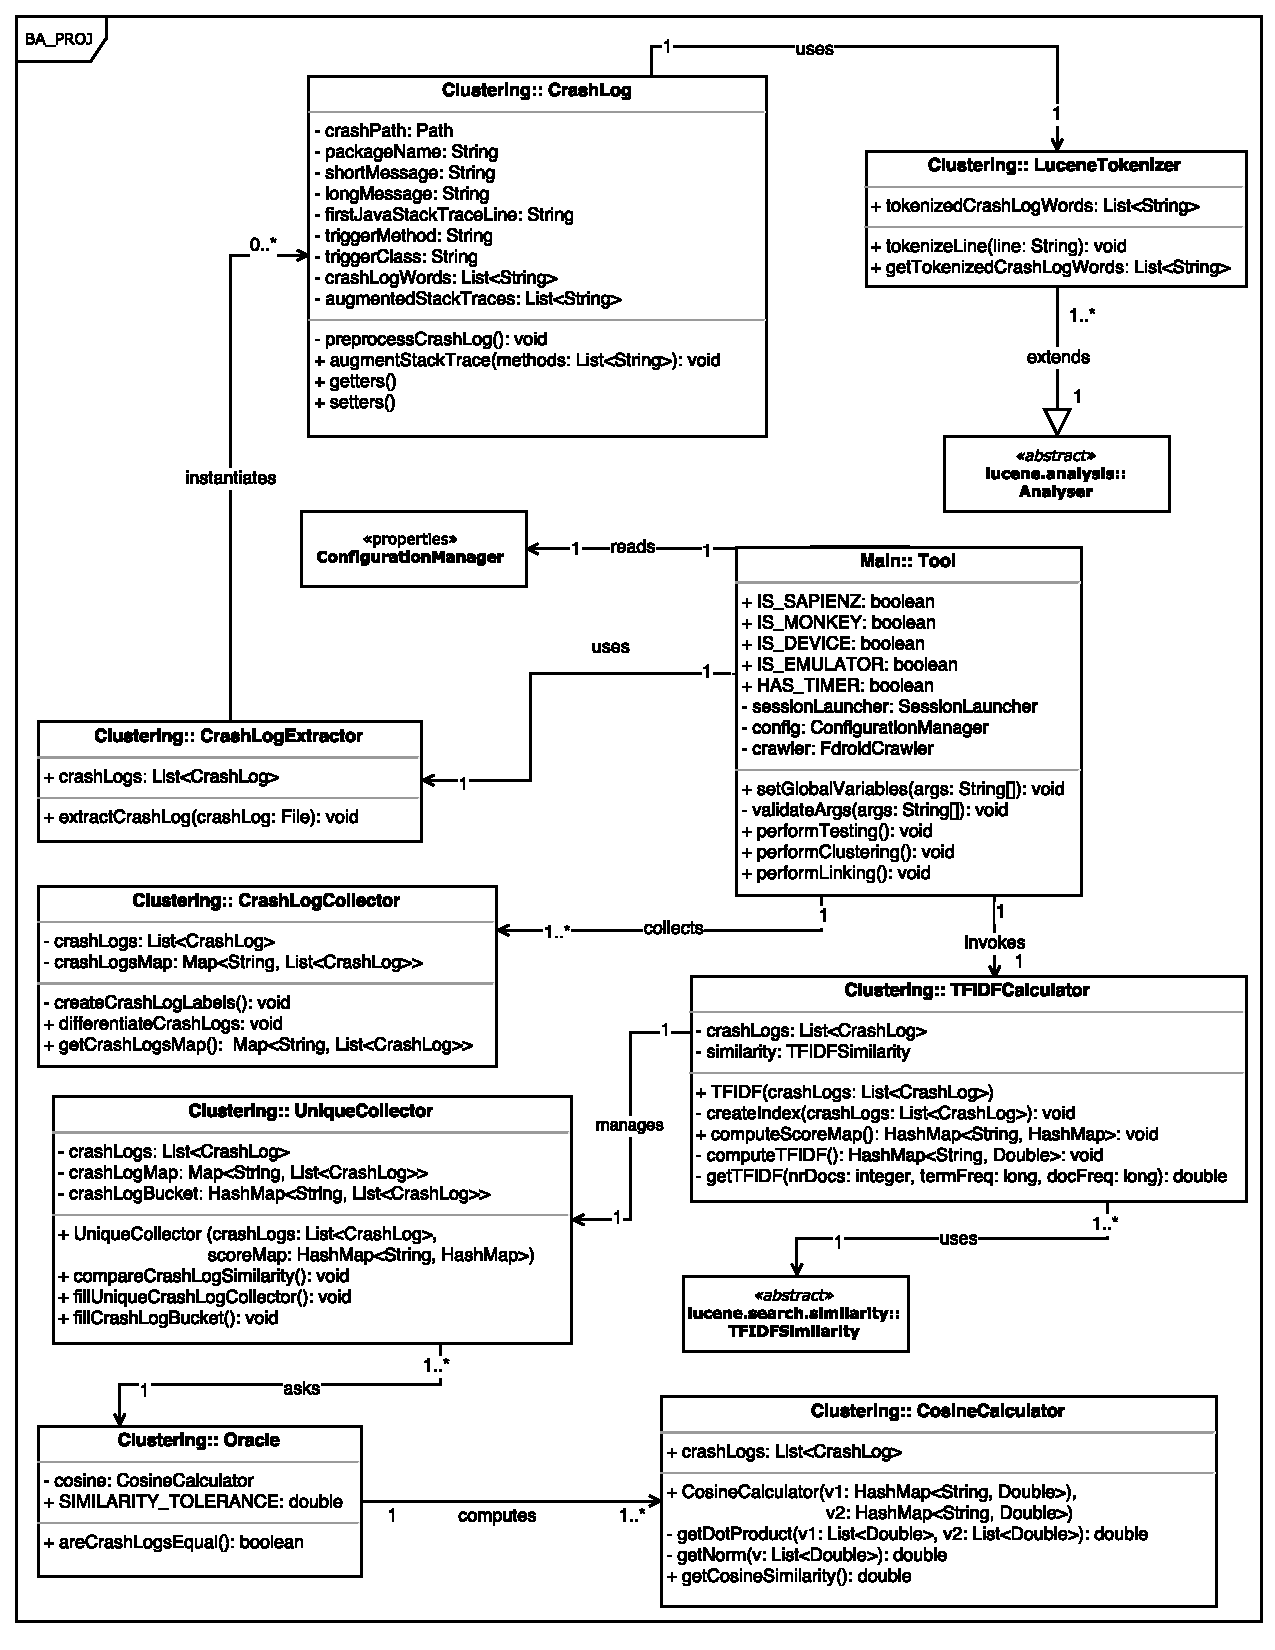
\includegraphics[width=\columnwidth]{diagrams/clustering.pdf} 
\caption{Class Diagram of the clustering part of the tool }
\label{clustering}
\vspace{-3mm} 
\end{figure}


\begin{figure}[t]
\centering 
%	\vspace{-1.5mm} 
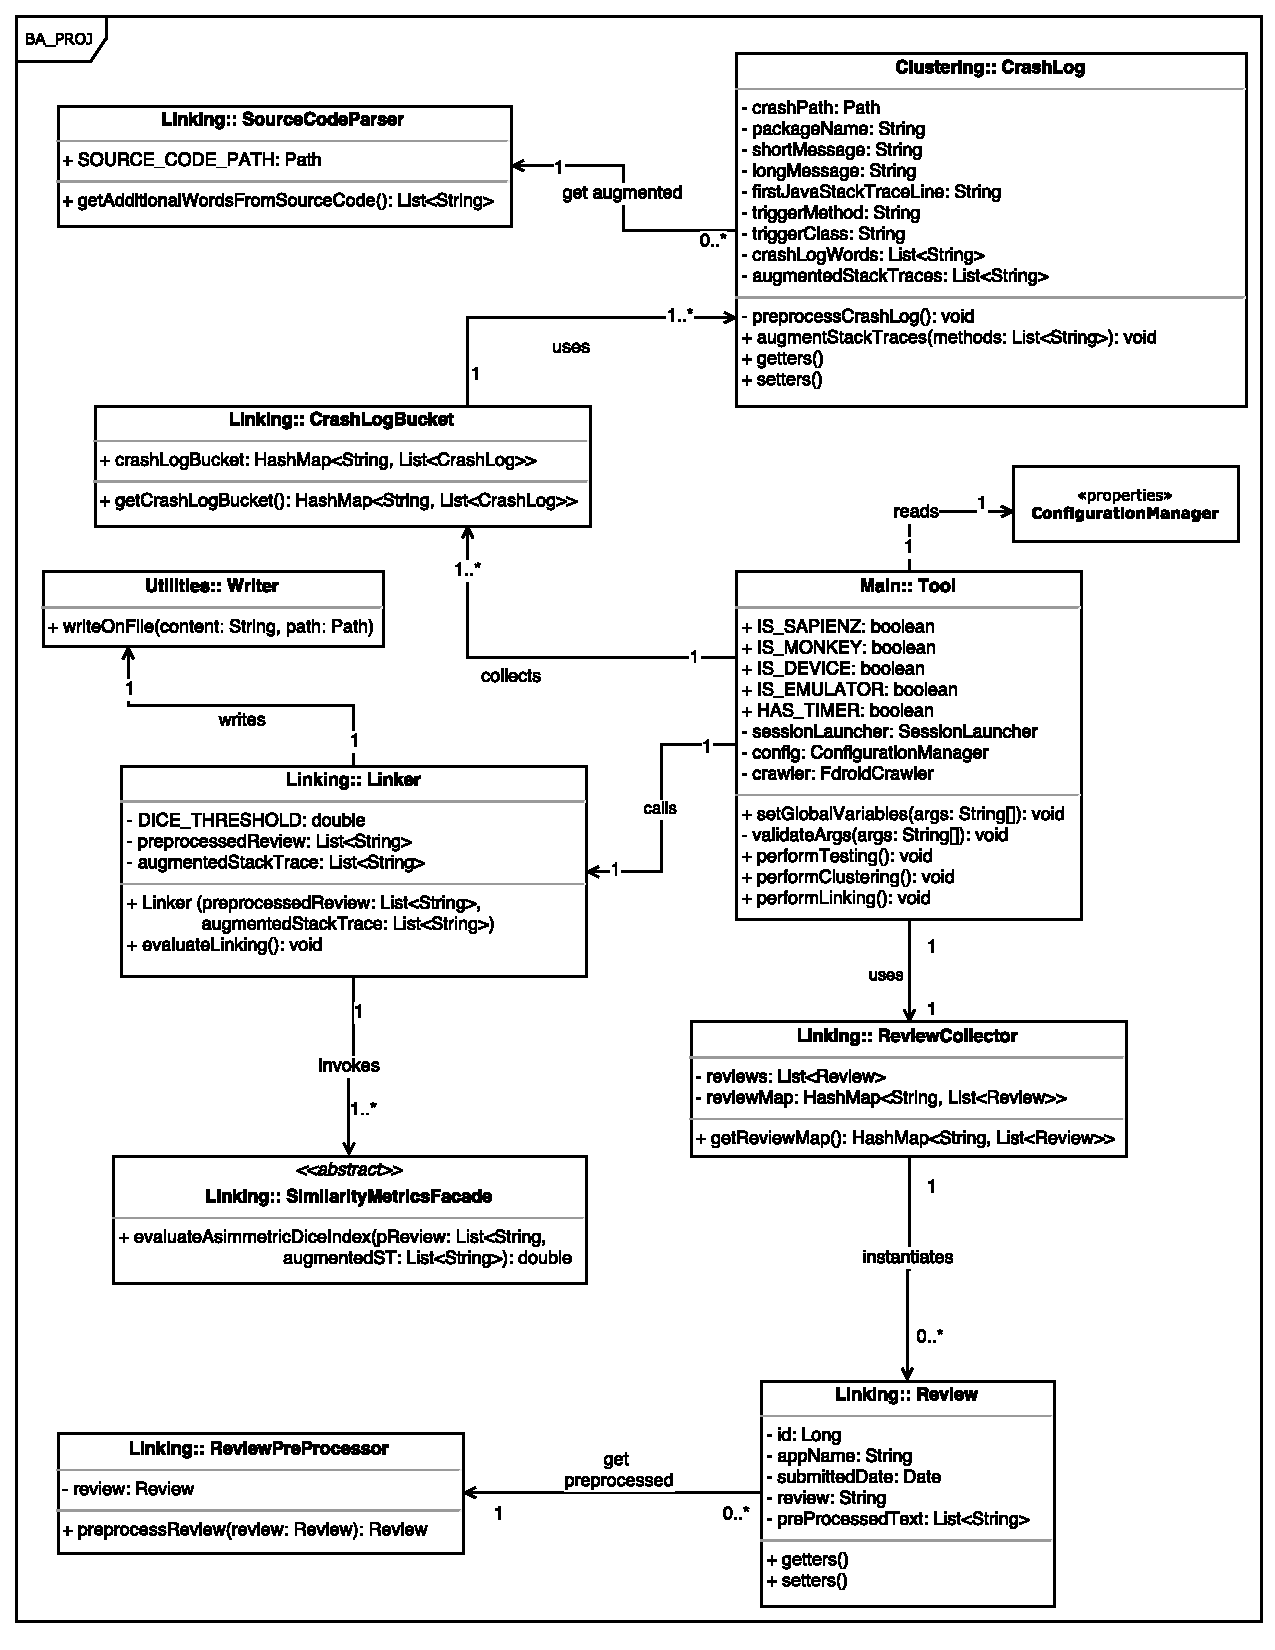
\includegraphics[width=\columnwidth]{diagrams/linking.pdf} 
\caption{Class Diagram of the linking part of the tool }
\label{linking}
\vspace{-3mm} 
\end{figure}